\documentclass[a4paper]{report}

\usepackage{cmap} % Улучшенный поиск русских слов в полученном pdf-файле
\usepackage[T2A]{fontenc} % Поддержка русских букв
\usepackage[utf8]{inputenc} % Кодировка utf8
\usepackage[english,russian]{babel} % Языки: русский, английский

% \usepackage{setspace}
% \onehalfspacing % Полуторный интервал

\frenchspacing
\usepackage{indentfirst} % Красная строка

%                30                    20           20
\usepackage[left=20mm, right=10mm, top=15mm, bottom=15mm]{geometry}

\usepackage{titlesec}
\titlespacing*{\chapter}{0pt}{-30pt}{8pt}
\titlespacing*{\section}{\parindent}{*4}{*4}
\titlespacing*{\subsection}{\parindent}{*4}{*4}
\titleformat{\chapter}{\LARGE\bfseries}{\thechapter}{20pt}{\LARGE\bfseries}
\titleformat{\section}{\Large\bfseries}{\thesection}{20pt}{\Large\bfseries}

\usepackage{amsmath}
\usepackage{amssymb}
\usepackage{commath}
\usepackage{icomma}

\usepackage[unicode,pdftex]{hyperref} % Ссылки в pdf
\hypersetup{hidelinks}

\usepackage{graphicx}

%% begin theorem
\usepackage{amsthm}

\makeatletter
\newtheoremstyle{indented}
	{}% measure of space to leave above the theorem
	{}% measure of space to leave below the theorem
	{}% name of font to use in the body of the theorem
	{\parindent}% measure of space to indent
	{\bfseries}% name of head font
	{.}% punctuation between head and body
	{ }% space after theorem head; " " = normal interword space
	{}% header specification (empty for default)
\makeatother

\theoremstyle{indented}

\newtheorem{definition}{Определение}[section]
\newtheorem{example}{Пример}[section]
\newtheorem{theorem}{Теорема}[section]
\newtheorem{task}{Задание}

\makeatletter
\DeclareRobustCommand\bfseriesitshape{%
	\not@math@alphabet\itshapebfseries\relax
	\fontseries\bfdefault
	\fontshape\itdefault
	\selectfont
}
\makeatother

\DeclareTextFontCommand{\textbfit}{\bfseriesitshape}
\DeclareTextFontCommand{\define}{\bfseriesitshape}
%% end theorem

%% begin columns
\usepackage{etoolbox,refcount}
\usepackage{multicol}

\newcounter{countitems}
\newcounter{nextitemizecount}
\newcommand{\setupcountitems}{%
	\stepcounter{nextitemizecount}%
	\setcounter{countitems}{0}%
	\preto\item{\stepcounter{countitems}}%
}
\makeatletter
\newcommand{\computecountitems}{%
	\edef\@currentlabel{\number\c@countitems}%
	\label{countitems@\number\numexpr\value{nextitemizecount}-1\relax}%
}
\newcommand{\nextitemizecount}{%
	\getrefnumber{countitems@\number\c@nextitemizecount}%
}
\newcommand{\previtemizecount}{%
	\getrefnumber{countitems@\number\numexpr\value{nextitemizecount}-1\relax}%
}
\makeatother
\newenvironment{AutoMultiColItemize}{%
	\ifnumcomp{\nextitemizecount}{>}{3}{\begin{multicols}{2}}{}%
		\setupcountitems\begin{itemize}}%
		{\end{itemize}%
		\unskip\computecountitems\ifnumcomp{\previtemizecount}{>}{3}{\end{multicols}}{}}
\makeatother
\newenvironment{AutoMultiColEnumerate}{%
	\ifnumcomp{\nextitemizecount}{>}{3}{\begin{multicols}{2}}{}%
		\setupcountitems\begin{enumerate}}%
		{\end{enumerate}%
		\unskip\computecountitems\ifnumcomp{\previtemizecount}{>}{3}{\end{multicols}}{}}
%% end columns


%% begin code
\usepackage{listings}
\usepackage{xcolor}

\lstdefinestyle{lispinline}{
	language=Lisp,
	backgroundcolor=\color{white},
	basicstyle=\footnotesize\ttfamily,
	keywordstyle=\color{blue},
	stringstyle=\color{red},
	commentstyle=\color{gray},
	tabsize=8,
	captionpos=b,
	breaklines=true,
	breakatwhitespace=true,
	escapeinside={\#*}{*)},
	morecomment=[l][\color{magenta}]{\#}
}

\newcommand{\code}[1]{\texttt{#1}}
%% end code

\usepackage{pgfplots}
\usetikzlibrary{datavisualization}
\usetikzlibrary{datavisualization.formats.functions}


\begin{document}

\begin{task}
	Представить следующие списки в виде списочных ячеек:
	\begin{AutoMultiColEnumerate}
		\item \code{'(open close halph)}
		\item \code{'((open1) (close2) (halph3))}
		\item \code{'((one) for all (and(me(for you))))}
		\item \code{'((TOOL) (call))}
		\item \code{'((TOOL1) ((call2)) ((sell)))}
		\item \code{'(((TOOL) (call)) ((sell)))}
	\end{AutoMultiColEnumerate}
\end{task}

\begin{figure}[!h]
	\begin{tabular}{|l|l|}
		\hline
		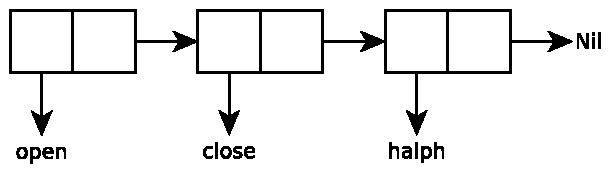
\includegraphics[scale=0.475]{inc/img/task0101.pdf} & 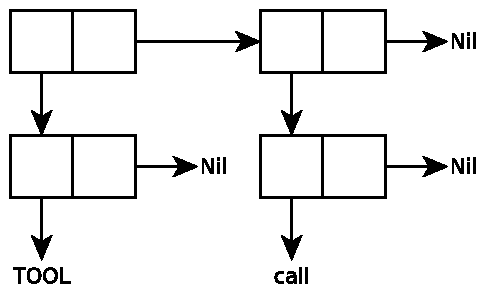
\includegraphics[scale=0.475]{inc/img/task0104.pdf} \\\hline
		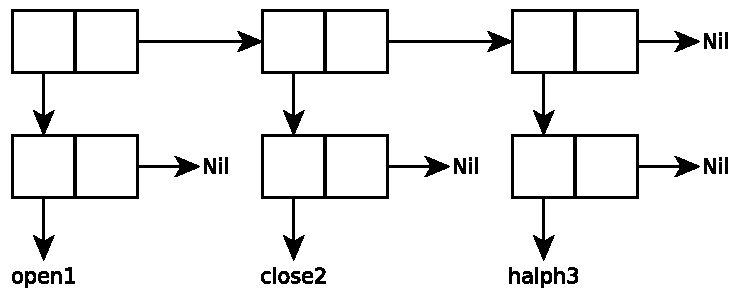
\includegraphics[scale=0.475]{inc/img/task0102.pdf} & 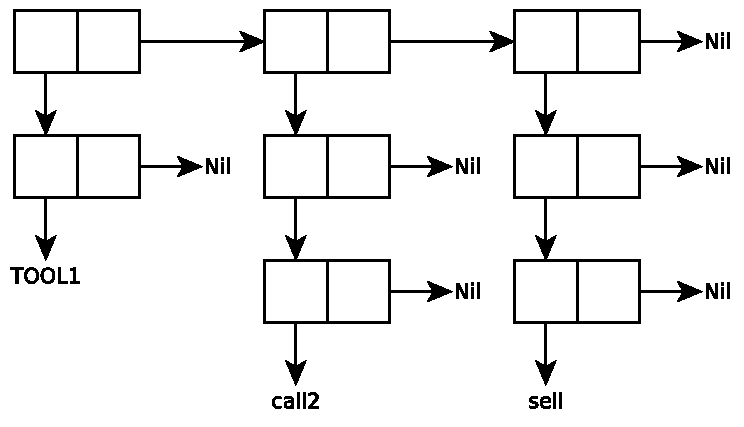
\includegraphics[scale=0.475]{inc/img/task0105.pdf} \\\hline
		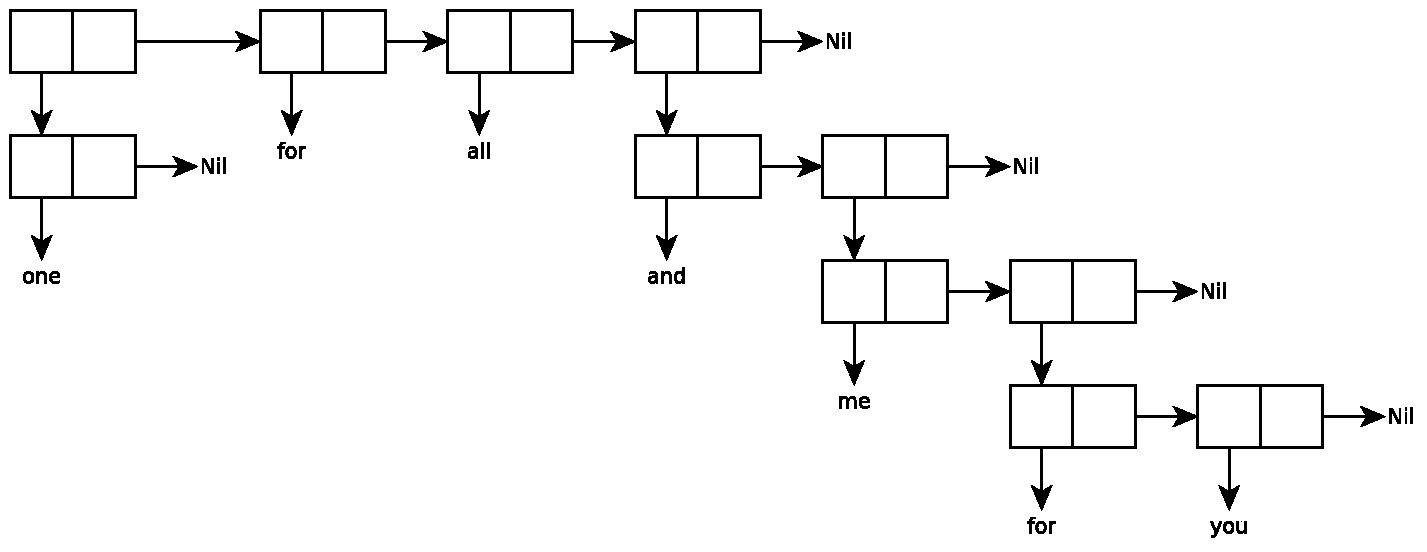
\includegraphics[scale=0.475]{inc/img/task0103.pdf} & 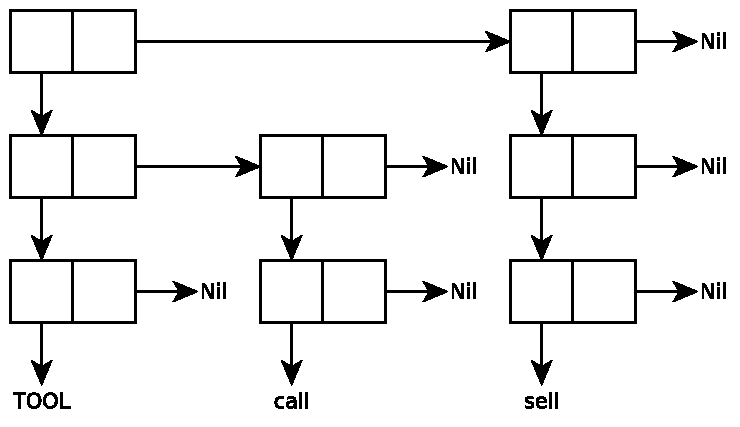
\includegraphics[scale=0.475]{inc/img/task0106.pdf} \\\hline
	\end{tabular}
\end{figure}

\begin{task}
	Используя только функции \code{CAR} и \code{CDR}, написать выражения, возвращающие 1) второй 2) третий 3) четвёртый элементы заданного списка.
\end{task}

\begin{AutoMultiColEnumerate}
	\item
\begin{lstlisting}[style=lispinline]
(car (cdr '(1 2 3 4 5)))             ; second
\end{lstlisting}

	\item
\begin{lstlisting}[style=lispinline]
(car (cdr (cdr '(1 2 3 4 5))))       ; third
\end{lstlisting}

	\item
\begin{lstlisting}[style=lispinline]
(car (cdr (cdr (cdr '(1 2 3 4 5))))) ; fourth
\end{lstlisting}
\end{AutoMultiColEnumerate}

\begin{task}
	Что будет в результате вычисления выражений?
	\begin{AutoMultiColEnumerate}
		\item
\begin{lstlisting}[style=lispinline]
(CAADR '((blue cude) (red pyramid))) ; red
\end{lstlisting}

		\item
\begin{lstlisting}[style=lispinline]
(CDAR '((abc) (def) (ghi)))          ; Nil
\end{lstlisting}

		\item
\begin{lstlisting}[style=lispinline]
(CADR '((abc) (def) (ghi)))          ; (def)
\end{lstlisting}

		\item
\begin{lstlisting}[style=lispinline]
(CADDR '((abc) (def) (ghi)))         ; (ghi)
\end{lstlisting}
	\end{AutoMultiColEnumerate}
\end{task}

\begin{task}
	Напишите результат вычисления выражений:
	\begin{AutoMultiColEnumerate}
		\item
\begin{lstlisting}[style=lispinline]
(list 'Fred 'and Wilma)
; The variable Wilma is unbound.
\end{lstlisting}

		\item
\begin{lstlisting}[style=lispinline]
(list 'Fred '(and Wilma))
; (Fred (and Wilma))
\end{lstlisting}

		\item
\begin{lstlisting}[style=lispinline]
(cons Nil Nil)
; (Nil)
\end{lstlisting}

		\item
\begin{lstlisting}[style=lispinline]
(cons T Nil)
; (T)
\end{lstlisting}

		\item
\begin{lstlisting}[style=lispinline]
(cons Nil T)
; (Nil . T)
\end{lstlisting}

		\item
\begin{lstlisting}[style=lispinline]
(list Nil)
; (Nil)
\end{lstlisting}

		\item
\begin{lstlisting}[style=lispinline]
(cons (T) Nil)
; The function T is undefined.
\end{lstlisting}

		\item
\begin{lstlisting}[style=lispinline]
(list '(one two) '(free temp))
; ((one two) (free temp))
\end{lstlisting}

		\item
\begin{lstlisting}[style=lispinline]
(cons 'Fred '(and Wilma))
; (Fred and Wilma)
\end{lstlisting}

		\item
\begin{lstlisting}[style=lispinline]
(cons 'Fred 'Wilma)
; (Fred . Wilma)
\end{lstlisting}

		\item
\begin{lstlisting}[style=lispinline]
(list Nil Nil)
; (Nil Nil)
\end{lstlisting}

		\item
\begin{lstlisting}[style=lispinline]
(list T Nil)
; (T Nil)
\end{lstlisting}

		\item
\begin{lstlisting}[style=lispinline]
(list Nil T)
; (Nil T)
\end{lstlisting}

		\item
\begin{lstlisting}[style=lispinline]
(cons T (list Nil))
; (T Nil)
\end{lstlisting}

		\item
\begin{lstlisting}[style=lispinline]
(list (T) Nil)
; The function T is undefined.
\end{lstlisting}

		\item
\begin{lstlisting}[style=lispinline]
(cons '(one two) '(free temp))
; ((one two) free temp)
\end{lstlisting}

	\end{AutoMultiColEnumerate}
\end{task}

\begin{task}
	Написать функцию \code{(f ar1 ar2 ar3 ar4)}, возвращающую список: \code{((ar1 ar2) (ar3 ar4))}.
	Написать функцию \code{(f ar1 ar2)}, возвращающую список: \code{((ar1) (ar2))}.
	Написать функцию \code{(f ar1)}, возвращающую список: \code{(((ar1)))}.
	Представить результаты в виде списочных ячеек.
\end{task}

\begin{lstlisting}[style=lispinline, frame=single]
(defun f (a1 a2 a3 a4)
	`((,a1 ,a2) (,a3 ,a4))
)

(defun f (a1 a2)
	`((,a1) (,a2))
)

(defun f (a1)
	`(((,a1)))
)
\end{lstlisting}

\begin{figure}[!h]
	\begin{tabular}{|l|l|l|}
		\hline
		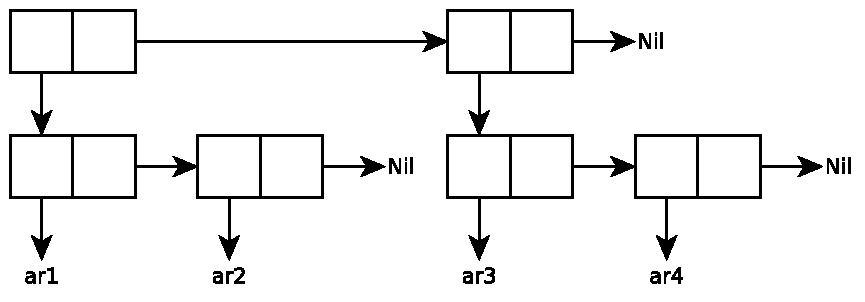
\includegraphics[scale=0.625]{inc/img/task0501.pdf} & 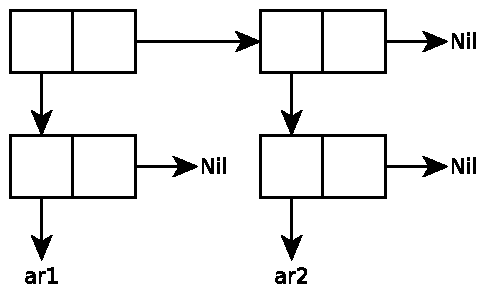
\includegraphics[scale=0.625]{inc/img/task0502.pdf} & 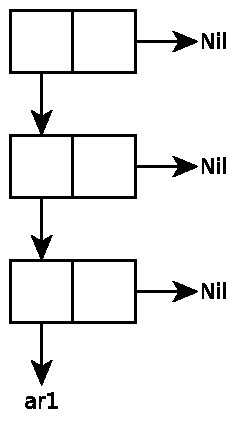
\includegraphics[scale=0.625]{inc/img/task0503.pdf} \\\hline
	\end{tabular}
\end{figure}

\end{document}
